%%%%%%%%%%%%%%%%%%%%%%%%%%%%%%%%%%%%%%%%%%%%%%%%%%%%%%%%%%%%%%%%%%%%%%%%%%%%%%%%
%% Plantilla de memoria en LaTeX para la ETSIT - Universidad Rey Juan Carlos
%%
%% Por Gregorio Robles <grex arroba gsyc.urjc.es>
%%     Grupo de Sistemas y Comunicaciones
%%     Escuela Técnica Superior de Ingenieros de Telecomunicación
%%     Universidad Rey Juan Carlos
%% (muchas ideas tomadas de Internet, colegas del GSyC, antiguos alumnos...
%%  etc. Muchas gracias a todos)
%%
%% La última versión de esta plantilla está siempre disponible en:
%%     https://github.com/gregoriorobles/plantilla-memoria
%%
%% Para obtener PDF, ejecuta en la shell:
%%   make
%% (las imágenes deben ir en PNG o JPG)

%%%%%%%%%%%%%%%%%%%%%%%%%%%%%%%%%%%%%%%%%%%%%%%%%%%%%%%%%%%%%%%%%%%%%%%%%%%%%%%%

\documentclass[a4paper, 12pt]{book}
%\usepackage[T1]{fontenc}

\usepackage[a4paper, left=2.5cm, right=2.5cm, top=3cm, bottom=3cm]{geometry}
\usepackage{times}
\usepackage[utf8]{inputenc}
\usepackage[spanish]{babel} % Comenta esta línea si tu memoria es en inglés
\usepackage{url}
%\usepackage[dvipdfm]{graphicx}
\usepackage{graphicx}
\usepackage{float}  %% H para posicionar figuras
\usepackage[nottoc, notlot, notlof, notindex]{tocbibind} %% Opciones de índice
\usepackage{latexsym}  %% Logo LaTeX
\usepackage{hyperref}
\usepackage{dirtree}
\usepackage{makecell}

\title{Memoria del Proyecto}
\author{Raúl Cano Montero}

\renewcommand{\baselinestretch}{1.5}  %% Interlineado

\begin{document}

\renewcommand{\refname}{Bibliografía}  %% Renombrando
\renewcommand{\appendixname}{Apéndice}

%%%%%%%%%%%%%%%%%%%%%%%%%%%%%%%%%%%%%%%%%%%%%%%%%%%%%%%%%%%%%%%%%%%%%%%%%%%%%%%%
% PORTADA

\begin{titlepage}
\begin{center}
\includegraphics[scale=0.8]{img/URJ_logo_Color_POS.png}

\vspace{1.75cm}

\Large
GRADO EN INGENIERÍA EN TECNOLOGÍAS DE LA TELECOMUNICACIÓN

\vspace{0.4cm}

\large
Curso Académico 2020/2021

\vspace{0.8cm}

Trabajo Fin de Grado

\vspace{2.5cm}

\LARGE
CREACIÓN AUTOMÁTICA DE PULL-REQUESTS A PARTIR DE RESULTADOS DE PYLINT

\vspace{4cm}

\large
Autor : Raúl Cano Montero \\
Tutor : Dr. Gregorio Robles
\end{center}
\end{titlepage}

\newpage
\mbox{}
\thispagestyle{empty} % para que no se numere esta pagina


%%%%%%%%%%%%%%%%%%%%%%%%%%%%%%%%%%%%%%%%%%%%%%%%%%%%%%%%%%%%%%%%%%%%%%%%%%%%%%%%
%%%% Para firmar
\clearpage
\pagenumbering{gobble}
\chapter*{}

\vspace{-4cm}
\begin{center}
\LARGE
\textbf{Trabajo Fin de Grado}

\vspace{1cm}
\large
Creación Automática de Pull-Requests a partir de Resultados de Pylint

\vspace{1cm}
\large
\textbf{Autor :} Raúl Cano Montero \\
\textbf{Tutor :} Dr. Gregorio Robles

\end{center}

\vspace{1cm}
La defensa del presente Proyecto Fin de Carrera se realizó el día \qquad$\;\,$ de julio de 2021, siendo calificada por el siguiente tribunal:


\vspace{0.5cm}
\textbf{Presidente:}

\vspace{1.2cm}
\textbf{Secretario:}

\vspace{1.2cm}
\textbf{Vocal:}


\vspace{1.2cm}
y habiendo obtenido la siguiente calificación:

\vspace{1cm}
\textbf{Calificación:}


\vspace{1cm}
\begin{flushright}
Fuenlabrada, a \qquad$\;\,$ de julio de 2021
\end{flushright}

%%%%%%%%%%%%%%%%%%%%%%%%%%%%%%%%%%%%%%%%%%%%%%%%%%%%%%%%%%%%%%%%%%%%%%%%%%%%%%%%
%%%% Dedicatoria

\chapter*{}
\pagenumbering{Roman} % para comenzar la numeracion de paginas en numeros romanos
\begin{flushright}
%TODO
\textit{Dedicado a \\
mi familia / mi abuelo / mi abuela}
\end{flushright}

%%%%%%%%%%%%%%%%%%%%%%%%%%%%%%%%%%%%%%%%%%%%%%%%%%%%%%%%%%%%%%%%%%%%%%%%%%%%%%%%
%%%% Agradecimientos

\chapter*{Agradecimientos}
%\addcontentsline{toc}{chapter}{Agradecimientos} % si queremos que aparezca en el índice
\markboth{AGRADECIMIENTOS}{AGRADECIMIENTOS} % encabezado 
%TODO
Aquí vienen los agradecimientos\ldots Aunque está bien acordarse de la pareja, no hay que olvidarse de dar las gracias a tu madre, que aunque a veces no lo parezca disfrutará tanto de tus logros como tú\ldots 
Además, la pareja quizás no sea para siempre, pero tu madre sí.

%%%%%%%%%%%%%%%%%%%%%%%%%%%%%%%%%%%%%%%%%%%%%%%%%%%%%%%%%%%%%%%%%%%%%%%%%%%%%%%%
%%%% Resumen

\chapter*{Resumen}
%\addcontentsline{toc}{chapter}{Resumen} % si queremos que aparezca en el índice
\markboth{RESUMEN}{RESUMEN} % encabezado
%TODO
Aquí viene un resumen del proyecto.
Ha de constar de tres o cuatro párrafos, donde se presente de manera clara y concisa de qué va el proyecto. 
Han de quedar respondidas las siguientes preguntas:

\begin{itemize}
  \item ¿De qué va este proyecto? ¿Cuál es su objetivo principal?
  \item ¿Cómo se ha realizado? ¿Qué tecnologías están involucradas?
  \item ¿En qué contexto se ha realizado el proyecto? ¿Es un proyecto dentro de un marco general?
\end{itemize}

Lo mejor es escribir el resumen al final.

%%%%%%%%%%%%%%%%%%%%%%%%%%%%%%%%%%%%%%%%%%%%%%%%%%%%%%%%%%%%%%%%%%%%%%%%%%%%%%%%
%%%% Resumen en inglés

\chapter*{Summary}
%\addcontentsline{toc}{chapter}{Summary} % si queremos que aparezca en el índice
\markboth{SUMMARY}{SUMMARY} % encabezado
%TODO
Here comes a translation of the ``Resumen'' into English. 
Please, double check it for correct grammar and spelling.
As it is the translation of the ``Resumen'', which is supposed to be written at the end, this as well should be filled out just before submitting.


%%%%%%%%%%%%%%%%%%%%%%%%%%%%%%%%%%%%%%%%%%%%%%%%%%%%%%%%%%%%%%%%%%%%%%%%%%%%%%%%
%%%%%%%%%%%%%%%%%%%%%%%%%%%%%%%%%%%%%%%%%%%%%%%%%%%%%%%%%%%%%%%%%%%%%%%%%%%%%%%%
% ÍNDICES %
%%%%%%%%%%%%%%%%%%%%%%%%%%%%%%%%%%%%%%%%%%%%%%%%%%%%%%%%%%%%%%%%%%%%%%%%%%%%%%%%

% Las buenas noticias es que los índices se generan automáticamente.
% Lo único que tienes que hacer es elegir cuáles quieren que se generen,
% y comentar/descomentar esa instrucción de LaTeX.

%%%% Índice de contenidos
\tableofcontents 
%%%% Índice de figuras
\cleardoublepage
\addcontentsline{toc}{chapter}{Lista de figuras} % para que aparezca en el indice de contenidos
\listoffigures % indice de figuras
%%%% Índice de tablas
\cleardoublepage
\addcontentsline{toc}{chapter}{Lista de tablas} % para que aparezca en el indice de contenidos
\listoftables % indice de tablas


%%%%%%%%%%%%%%%%%%%%%%%%%%%%%%%%%%%%%%%%%%%%%%%%%%%%%%%%%%%%%%%%%%%%%%%%%%%%%%%%
%%%%%%%%%%%%%%%%%%%%%%%%%%%%%%%%%%%%%%%%%%%%%%%%%%%%%%%%%%%%%%%%%%%%%%%%%%%%%%%%
% INTRODUCCIÓN %
%%%%%%%%%%%%%%%%%%%%%%%%%%%%%%%%%%%%%%%%%%%%%%%%%%%%%%%%%%%%%%%%%%%%%%%%%%%%%%%%

\cleardoublepage
\chapter{Introducción}
\label{sec:intro} % etiqueta para poder referenciar luego en el texto con ~\ref{sec:intro}
\pagenumbering{arabic} % para empezar la numeración de página con números
%TODO
En este capítulo se introduce el proyecto.
Debería tener información general sobre el mismo, dando la información sobre el contexto en el que se ha desarrollado.

No te olvides de echarle un ojo a la página con los cinco errores de escritura más frecuentes\footnote{\url{http://www.tallerdeescritores.com/errores-de-escritura-frecuentes}}.

Aconsejo a todo el mundo que mire y se inspire en memorias pasadas.
Las memorias de los proyectos que he llevado yo están (casi) todas almacenadas en mi web del GSyC\footnote{\url{https://gsyc.urjc.es/~grex/pfcs/}}.

\section{Sección}
\label{sec:seccion}

Esto es una sección, que es una estructura menor que un capítulo. 

Por cierto, a veces me comentáis que no os compila por las tildes.
Eso es un problema de codificación.
Al guardar el archivo, guardad la codificación de ``ISO-Latin-1'' a ``UTF-8'' (o viceversa) y funcionará.

\subsection{Estilo}
\label{subsec:estilo}

Recomiendo leer los consejos prácticos sobre escribir documentos científicos en \LaTeX \ de Diomidis Spinellis\footnote{\url{https://github.com/dspinellis/latex-advice}}.

Lee sobre el uso de las comas\footnote{\url{http://narrativabreve.com/2015/02/opiniones-de-un-corrector-de-estilo-11-recetas-para-escribir-correctamente-la-coma.html}}. 
Las comas en español no se ponen al tuntún.
Y nunca, nunca entre el sujeto y el predicado (p.ej. en ``Yo, hago el TFG'' sobre la coma).
La coma no debe separar el sujeto del predicado en una oración, pues se cortaría la secuencia natural del discurso.
No se considera apropiado el uso de la llamada coma respiratoria o \emph{coma criminal}.
Solamente se suele escribir una coma para marcar el lugar que queda cuando omitimos el verbo de una oración, pero es un caso que se da de manera muy infrecuente al escribir un texto científico (p.ej. ``El Real Madrid, campeón de Europa'').

A continuación, viene una figura, la Figura~\ref{figura:foro_hilos}. 
Observarás que el texto dentro de la referencia es el identificador de la figura (que se corresponden con el ``label'' dentro de la misma). 
También habrás tomado nota de cómo se ponen las ``comillas dobles'' para que se muestren correctamente. 
Nota que hay unas comillas de inicio (``) y otras de cierre (''), y que son diferentes.
Volviendo a las referencias, nota que al compilar, la primera vez se crea un diccionario con las referencias, y en la segunda compilación se ``rellenan'' estas referencias. 
Por eso hay que compilar dos veces tu memoria.
Si no, no se crearán las referencias.

 \begin{figure}
    \centering
    \includegraphics[bb=0 0 800 600, width=12cm, keepaspectratio]{img/foro1}
    \caption{Página con enlaces a hilos}
    \label{figura:foro_hilos}
 \end{figure}

A continuación un bloque ``verbatim'', que se utiliza para mostrar texto tal cual.
Se puede utilizar para ofrecer el contenido de correos electrónicos, código, entre otras cosas.

{\footnotesize
\begin{verbatim}
    From gaurav at gold-solutions.co.uk  Fri Jan 14 14:51:11 2005
    From: gaurav at gold-solutions.co.uk (gaurav_gold)
    Date: Fri Jan 14 19:25:51 2005
    Subject: [Mailman-Users] mailman issues
    Message-ID: <003c01c4fa40$1d99b4c0$94592252@gaurav7klgnyif>

    Dear Sir/Madam,
    How can people reply to the mailing list?  How do i turn off
    this feature? How can i also enable a feature where if someone
    replies the newsletter the email gets deleted?
    Thanks

    From msapiro at value.net  Fri Jan 14 19:48:51 2005
    From: msapiro at value.net (Mark Sapiro)
    Date: Fri Jan 14 19:49:04 2005
    Subject: [Mailman-Users] mailman issues
    In-Reply-To: <003c01c4fa40$1d99b4c0$94592252@gaurav7klgnyif>
    Message-ID: <PC173020050114104851057801b04d55@msapiro>

    gaurav_gold wrote:
    >How can people reply to the mailing list?  How do i turn off
    this feature? How can i also enable a feature where if someone
    replies the newsletter the email gets deleted?

    See the FAQ
    >Mailman FAQ: http://www.python.org/cgi-bin/faqw-mm.py
    article 3.11
\end{verbatim}
}

\section{Estructura de la memoria}
\label{sec:estructura}
%TODO
En esta sección se debería introducir la esctura de la memoria. 

Así:

\begin{itemize}
  \item En el primer capítulo se hace una intro al proyecto.
  
  \item En el capítulo~\ref{chap:objetivos} (ojo, otra referencia automática) se muestran los objetivos del proyecto.
  
  \item A continuación se presenta el estado del arte en el capítulo~\ref{chap:estado}.
  
  \item \ldots
\end{itemize}



%%%%%%%%%%%%%%%%%%%%%%%%%%%%%%%%%%%%%%%%%%%%%%%%%%%%%%%%%%%%%%%%%%%%%%%%%%%%%%%%
%%%%%%%%%%%%%%%%%%%%%%%%%%%%%%%%%%%%%%%%%%%%%%%%%%%%%%%%%%%%%%%%%%%%%%%%%%%%%%%%
% OBJETIVOS %
%%%%%%%%%%%%%%%%%%%%%%%%%%%%%%%%%%%%%%%%%%%%%%%%%%%%%%%%%%%%%%%%%%%%%%%%%%%%%%%%

\cleardoublepage % empezamos en página impar
\chapter{Objetivos} % título del capítulo (se muestra)
\label{chap:objetivos} % identificador del capítulo (no se muestra, es para poder referenciarlo)

\section{Objetivo general} % título de sección (se muestra)
\label{sec:objetivo-general} % identificador de sección (no se muestra, es para poder referenciarla)

El objetivo de este Trabajo de Fin de Grado es realizar el análisis, mediante la herramienta Pylint, la corrección del código y la creación de Pull-Requests sobre proyectos desarrollados en Python y almacenados en GitHub, para que éstos cumplan con las normas recogidas en la guía de estilo de Python denominada PEP8

\section{Objetivos específicos}
\label{sec:objetivos-especificos}

Para poder cumplir con el objetivo general se han tenido en cuenta los siguientes objetivos específicos:

\begin{itemize}
	\item \textbf{Trabajar con proyectos reales.} Utilizar la aplicación para analizar y corregir proyectos reales.
	\item \textbf{Aplicación web.} Desarrollar como una aplicación web para hacer mejor y más sencilla la experiencia de usuario.
	\item \textbf{Accesibilidad desde Internet.} Hacer que la aplicación esté en funcionamiento continuamente y sea accesible desde cualquier ubicación.
	\item \textbf{Compatibilidad con el servidor GitLab de la ETSIT.} Hacer que la aplicación sea compatible con el GitLab de la ETSIT para permitir que los alumnos de la escuela puedan analizar y corregir sus proyectos.
	\item \textbf{Análisis de aceptación de las Pull-Requests.} Evaluar la aceptación de los cambios realizados en los proyectos mediante el análisis del estado de las Pull-Requests realizadas.
\end{itemize}


\section{Planificación temporal}
\label{sec:planificacion-temporal}
%TODO
A mí me gusta que aquí pongáis una descripción de lo que os ha llevado realizar el trabajo.
Hay gente que añade un diagrama de GANTT.
Lo importante es que quede claro cuánto tiempo llevas (tiempo natural, p.ej., 6 meses) y a qué nivel de esfuerzo (p.ej., principalmente los fines de semana).


%%%%%%%%%%%%%%%%%%%%%%%%%%%%%%%%%%%%%%%%%%%%%%%%%%%%%%%%%%%%%%%%%%%%%%%%%%%%%%%%
%%%%%%%%%%%%%%%%%%%%%%%%%%%%%%%%%%%%%%%%%%%%%%%%%%%%%%%%%%%%%%%%%%%%%%%%%%%%%%%%
% ESTADO DEL ARTE %
%%%%%%%%%%%%%%%%%%%%%%%%%%%%%%%%%%%%%%%%%%%%%%%%%%%%%%%%%%%%%%%%%%%%%%%%%%%%%%%%

\cleardoublepage
\chapter{Estado del arte}
\label{chap:estado}

En este capítulo se describen brevemente las principales tecnologías utilizadas en el desarrollo del proyecto.

\section{Python} 
\label{sec:python}
Python \cite{python} es un lenguaje de programación Open Source escrito por Guido van Rossum entre finales de los años 80 y principios de los 90. El objetivo de la creación de Python era tener un lenguaje de programación con una sintaxis sencilla, como el lenguaje ABC en el que se inspira, añadiendo la posibilidad de realizar llamadas al sistema con compatibilidad con distintos sistemas operativos.

Python es un lenguaje de programación interpretado, interactivo y orientado a objetos. Al ser un lenguaje interpretado se reduce el tiempo entre la escritura del código y la ejecución del mismo, ya que no hay que compilarlo cada vez que se realice una modificación del código. Sin embargo, ésto implica que sea necesaria la instalación de un intérprete en la máquina que va a ejecutar el código y aumenta el tiempo de la ejecución respecto a los lenguajes compilados.

Python incorpora módulos, excepciones, tipado dinámico, tipos de datos dinámicos de muy alto nivel y clases. La librería estándar de Python le permite cubrir distintas áreas, como el procesamiento de cadenas de texto, protocolos de red, ingeniería del software e interacción con el sistema operativo.

Además de la programación orientada a objetos, soporta múltiples paradigmas de programación como la programación procedimental y la programación funcional y también es compatible con diversos sistemas operativos, incluyendo Windows y múltiples variantes de Unix, como Linux y macOS.

Actualmente Python es uno de los lenguajes de programación más utilizados~\cite{stackoverflowsurvey}.

\section{PEP 8} 
\label{sec:pep8}
Python Enhancement Proposal 8, más conocida como PEP 8~\cite{pep8}, es una guía de estilo para código escrito en Python que contiene recomendaciones y convenciones dirigidas a mejorar la consistencia y legibilidad del código.
Algunas de las convenciones indicadas por PEP 8 son las siguientes:
\begin{itemize}
	\item \textbf{Tabulación}: Se debe tabular utilizando 4 espacios por cada nivel de tabulación.
	\item \textbf{Caracteres por línea}: Cada línea de código debe tener, como máximo, una longitud de 79 caracteres.
	\item \textbf{Imports}: Los módulos adicionales deben ser importados al inicio de cada fichero y sólo debe haber uno por línea.
	\item \textbf{Espacios antes y después de operadores}: Antes y después de cada operador debe haber un único espacio.
	\item \textbf{Nomenclatura}: Cada elemento tiene definidas unas normas distintas al realizar su declaración.
\end{itemize}

PEP 8 también nos indica que las distintas normas pueden ser ignoradas en determinados casos como, por ejemplo:
\begin{itemize}
	\item Cuando se añade código a una librería ya existente que sigue un estilo distinto se debe respetar dicho estilo para mantener la consistencia dentro de dicha librería.
	\item En caso de que el código necesite funcionar en versiones antiguas de Python y modificarlo suponga una incompatibilidad.
	\item Cuando modificar el código dificulte la lectura y comprensión del mismo. 
\end{itemize}

\section{Pylint} 
\label{sec:pylint}
Pylint~\cite{pylint} es una herramienta de análisis de código escrito en Python que comprueba si hay incumplimiento de la guía de estilo PEP 8. Es un analizador de código estático, lo que facilita el análisis del código ya que se realiza sin tener que ejecutarlo.

La salida de Pylint muestra para cada error detectado en qué fichero, línea y columna se ha encontrado y, al final de la salida, una calificación del código analizado en función de los errores que se han detectado. El formato de esta salida y las opciones del análisis, como los errores que deben buscarse o los ficheros que deben analizarse, son configurables mediante argumentos introducidos al ejecutar la herramienta o mediante un fichero de configuración llamado pylintrc.

\section{Django} 
\label{sec:django}
Django\cite{django} es un framework de desarrollo de aplicaciones web de código abierto escrito en Python. Django está basado en una variación de la arquitectura MVC (Model-View-Controller) a la que denominan MVT (Model-View-Template):
\begin{itemize}
	\item \textbf{Model}: Datos con los que el sistema trabaja. Se definen en el fichero models.py.
	\item \textbf{View}: Describe qué datos se presentan mediante los ficheros views.py y urls.py. 
	\item \textbf{Template}: Definido por las plantillas HTML y CSS que describen cómo se presentan los datos.
\end{itemize}

\section{PostgreSQL} 
\label{sec:postgresql}

PostgreSQL~\cite{postgresql} es un sistema de gestión de bases de datos relacionales de código abierto basado en POSTGRES. PostgreSQL es compatible con gran parte del estándar SQL, añade algunas características propias, como el control de concurrencias multiversión o la compatibilidad con consultas complejas, y permite al usuario añadir nuevos tipos de datos, funciones u operadores.

\section{HTML} 
\label{sec:html}

HTML (Hypertext Markup Language)~\cite{htmlcss} es el lenguaje de marcado estándar para la creación de páginas web. Este estándar está a cargo del World Wide Web Consortium (W3C) y es compatible con todos los navegadores web.
Con HTML se define la estructura de las páginas web mediante la utilización de distintas etiquetas.

\section{CSS} 
\label{sec:css}

CSS (Cascading Style Sheets)~\cite{htmlcss} es un lenguaje de diseño web utilizado para definir la apariencia y el estilo visual de una página web. Al igual que HTML, es un estándar a cargo del World Wide Web Consortium (W3C).
CSS establece cómo se muestran los elementos declarados en un documento HTML definiendo propiedades como los colores, fuentes y diseño. Para ello CSS hace uso de reglas, formadas por selectores, que indican sobre qué elementos HTML se aplican, y declaraciones, que definen y modifican las propiedades.
CSS es independiente de HTML y se puede llevar a cabo desde un fichero separado, lo que facilita el mantenimiento y la reutilización de las hojas de estilo.


\section{Bootstrap} 
\label{sec:bootstrap}

Bootstrap~\cite{bootstrap} es un framework de código abierto dirigido al desarrollo front-end de páginas web. Es una biblioteca que contiene herramientas HTML, CSS y JavaScript que facilitan el diseño y ayudan a realizar modificaciones de manera más sencilla en el estilo visual. Bootstrap contiene plantillas predefinidas con diferentes estilos de botones, formularios, desplegables o pestañas, entre otros componentes. Una de las características más importantes de Bootstrap es que también aporta el diseño responsive, que adapta automáticamente la presentación de la página web a diferentes tipos de dispositivos teniendo en cuenta el tamaño de pantalla y la resolución, lo que facilita la visualización y aumenta la compatibilidad de las páginas web.

\section{JavaScript} 
\label{sec:javascript}

JavaScript~\cite{javascript} es un lenguaje de programación interpretado, orientado a objetos, imperativo, multiparadigma, de tipado débil y dinámico y basado en prototipos. Tiene una sintaxis inspirada en la de Java y C++, con sentencias que funcionan igual que en esos lenguajes.
Su uso principal es el scripting en páginas web dirigido a establecer el comportamiento de éstas al suceder un evento determinado. La ejecución de estos scripts se realiza en el lado del cliente, en el navegador web, sin tener acceso al lado del servidor.
El uso de JavaScript está ampliamente extendido debido a que es compatible con cualquier navegador y sistema operativo.

\section{jQuery} 
\label{sec:jquery}

jQuery~\cite{jquery} es una librería de JavaScript de código abierto que simplifica la interacción entre JavaScript y HTML. jQuery facilita la manipulación del HTML, el manejo de eventos, el desarrollo de animaciones y el uso de AJAX y es compatible con cualquier navegador web y sistema operativo actual.

\section{Chart.js} 
\label{sec:chartjs}

Chart.js~\cite{chartjs} es una librería de JavaScript de código abierto dirigida a la representación y visualización de datos. Permite generar gráficos de distintos tipos, como barras, líneas, circulares o de dispersión, entre otros, y personalizar cómo se muestran dichos gráficos.
Actualmente es una de las librerías de visualización de datos en JavaScript más populares en GitHub.

\section{JSON} 
\label{sec:json}

JSON~\cite{json} (JavaScript Object Notation) es un formato de intercambio de datos fácil de leer y escribir para humanos y fácil de generar e interpretar para las máquinas. Como su nombre indica, está basado en la sintaxis de objetos de JavaScript, teniendo una estructura formada por pares de nombre/valor.
JSON es independiente de cualquier lenguaje y, por ello, es compatible con la gran mayoría de los lenguajes de programación actuales.

\section{API-REST} 
\label{sec:api}

Una API (Application Programming Interface) es un conjunto de instrucciones y protocolos ofrecidos por determinadas aplicaciones para dar acceso a su propia información o funciones. La API actúa como intermediario entre la propia aplicación y el solicitante y devuelve a éste último una respuesta con el resultado de la operación realizada o con la información solicitada.

Una API REST es un tipo de API en el que el acceso está basado en arquitectura REST (Representational State Transfer), por lo que las llamadas a dicha API se llevan a cabo mediante peticiones HTTP y el uso de objetos XML o JSON.

\section{Git} 
\label{sec:git}

Git\cite{git} es un software de código abierto de control de versiones diseñado por Linus Torvald para facilitar la gestión y el trabajo en equipo en proyectos de desarrollo de software.
Para un proyecto almacenado en un repositorio, Git permite que cada integrante del equipo tenga una versión en local del proyecto y vaya subiendo sus modificaciones al repositorio.

El funcionamiento de Git se basa en la creación, uso y mezcla de ramas dentro del proyecto, existiendo una rama principal, conocida como master, y creándose ramas secundarias para realizar las modificaciones en el código. Una vez se realicen las modificaciones, la rama secundaria se mezcla con la rama master y cuando otros miembros del equipo actualicen su rama master descargarán los cambios realizados sin que esto afecte a su trabajo.

\section{GitHub} 
\label{sec:github}

GitHub~\cite{github} es un servicio web, propiedad de Microsoft, que almacena repositorios de proyectos de desarrollo software que utilizan el sistema de control de versiones Git. Permite la creación de repositorios públicos, que podrán ser vistos y descargados por cualquier usuario, y repositorios privados, que únicamente serán visibles por los colaboradores de dicho repositorio.
Cualquier usuario puede colaborar en proyectos públicos mediante la creación de Pull-Requests. De esta manera un usuario externo al proyecto puede sugerir al propietario de un repositorio que realice los cambios indicados en un proyecto, mientras que el usuario propietario puede decidir aceptar o no las modificaciones realizadas.
Es la plataforma de almacenamiento de repositorios más usada.

\section{GitLab} 
\label{sec:gitlab}

GitLab~\cite{gitlab} es un servicio web de código abierto que almacena repositorios de proyectos de desarrollo software que utilizan el sistema de control de versiones Git. Al igual que GitHub, permite la creación de repositorios públicos y privados y tiene un sistema de Pull-Requests que, en este caso, se denominan Merge-Requests.
GitLab permite la instalación en un servidor privado para no hacer uso de la plataforma pública que se encuentra abierta a todo el mundo.

\section{Heroku} 
\label{sec:Heroku}

Heroku~\cite{heroku} es una plataforma como servicio (PaaS) que permite alojar aplicaciones en la nube. Es compatible con aplicaciones desarrolladas en Node.js, Ruby, Python, Java, PHP, Go, Scala y Clojure y con bases de datos PostgreSQL, MongoDB y Redis.

%%%%%%%%%%%%%%%%%%%%%%%%%%%%%%%%%%%%%%%%%%%%%%%%%%%%%%%%%%%%%%%%%%%%%%%%%%%%%%%%
%%%%%%%%%%%%%%%%%%%%%%%%%%%%%%%%%%%%%%%%%%%%%%%%%%%%%%%%%%%%%%%%%%%%%%%%%%%%%%%%
% DISEÑO E IMPLEMENTACIÓN %
%%%%%%%%%%%%%%%%%%%%%%%%%%%%%%%%%%%%%%%%%%%%%%%%%%%%%%%%%%%%%%%%%%%%%%%%%%%%%%%%

\cleardoublepage
\chapter{Diseño e implementación}

En este capítulo se describe de manera detallada el diseño y la implementación del proyecto.

\section{Arquitectura general} 
\label{sec:arquitectura}

La arquitectura de la aplicación se basa en el modelo cliente-servidor representado en la figura~\ref{fig:cliente-servidor}.
En este modelo existen dos partes diferenciadas: cliente y servidor.

Cliente y servidor puede encontrarse en la misma máquina, pero en el caso de este proyecto siempre van a estar en máquinas separadas, ya que la aplicación se encuentra desplegada en Heroku y la comunicación entre ambas partes se lleva a cabo a través de internet mediante protocolo HTTP.

\begin{figure}
  \centering
  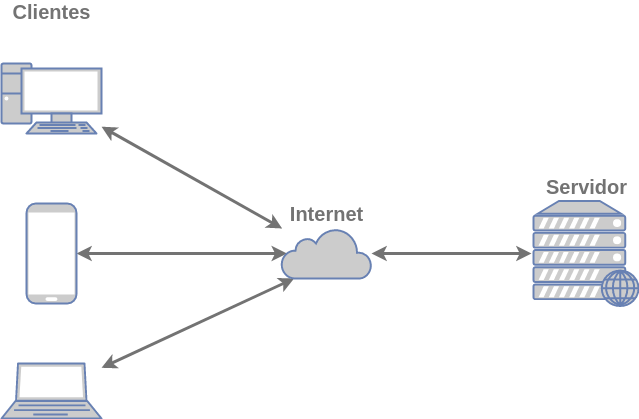
\includegraphics[width=9cm, keepaspectratio]{img/cliente-servidor.png}
  \caption{Modelo cliente-servidor.}\label{fig:cliente-servidor}
\end{figure}

\subsection{Cliente}
\label{subsec:arq_cliente}

La parte cliente está formada por el navegador web desde el que el usuario accede a la aplicación. 
El navegador recibe la página web en forma de código HTML y lo interpreta para mostrarlo al usuario para su interacción.
Las acciones que el usuario lleve a cabo sobre la página web son convertidas en peticiones HTTP por el navegador web y se envían al servidor, que las procesa y devuelve una respuesta al cliente en forma de código HTML.
Desde la parte cliente no se realiza ninguna ejecución a excepción de los scripts JavaScript que puedan encontrarse dentro del HTML.

\subsection{Servidor}
\label{subsec:arq_servidor}

La parte servidor está desplegada en Heroku y contiene la aplicación desarrollada en Django y una base de datos PostgreSQL tal y como se ve reflejado en la figura~\ref{fig:servidor}.

El servidor desplegado en Heroku recibe las peticiones HTTP realizadas sobre una determinada URL y Django las procesa realizando las acciones correspondientes para la petición recibida y, si es necesario, realiza una consulta a la base de datos PostgreSQL pudiendo ser ésta para obtener o modificar datos almacenados en dicha base de datos.
Por último, el servidor devuelve al cliente el código HTTP con la respuesta a la petición realizada.
\newline
\begin{figure}[h]
  \centering
  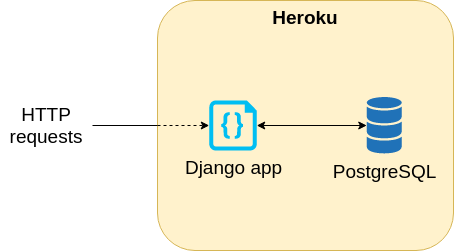
\includegraphics[width=9cm, keepaspectratio]{img/servidor.png}
  \caption{Arquitectura del servidor.}\label{fig:servidor}
\end{figure}

\section{Diseño e implementación del servidor} 
\label{sec:diseno_servidor}

El funcionamiento global de la aplicación y sus etapas son las representadas en la figura~\ref{fig:uso}.

El inicio del uso de la aplicación es la introducción en un formulario de la URL del repositorio que se va analizar. Una vez comprobado que la URL introducida apunta a un repositorio, se descargan los datos del mismo y se lleva a cabo la primera de las etapas principales, el análisis del código mediante la utilización de Pylint.
Una vez se ha analizado el código y se ha confirmado que se quieren llevar a cabo las modificaciones correspondientes a los errores detectados por Pylint, se realiza un fork del repositorio, se descarga el código de dicho fork y se realiza la segunda etapa principal, la corrección de los errores.
Cuando se ha terminado con la corrección se llega al final del proceso con la realización de una Pull-Request/Merge-Request con las modificaciones realizada en el código.

\begin{figure}[h]
  \centering
  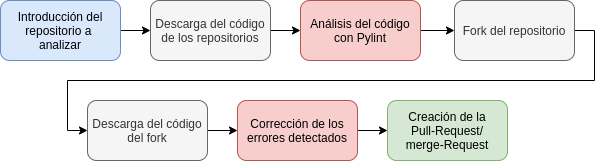
\includegraphics[width=12cm, keepaspectratio]{img/uso.png}
  \caption{Etapas del uso de la aplicación.}\label{fig:uso}
\end{figure}

\subsection{Django}
\label{subsec:diseño_django}

Como ya se ha explicado en la sección~\ref{sec:django}, Django se basa en una arquitectura MVT como la representada en la figura~\ref{fig:django}.

Las peticiones HTTP son procesadas por la parte \textit{Views} que realiza las acciones correspondientes y, si es necesario, se comunica \textit{Model} para obtener o modificar la información almacenada en la base de datos.
Una vez realizado el procesamiento, es la parte \textit{Templates} la que se encarga de construir la respuesta HTTP a partir de los datos proporcionados por \textit{Views} y las plantillas HTML.

Esta respuesta HTTP es enviada de vuelta al cliente, que visualiza la página construida por \textit{Templates}, mostrando los datos de \textit{Model} que han sido procesados por \textit{Views}.

\begin{figure}[h]
  \centering
  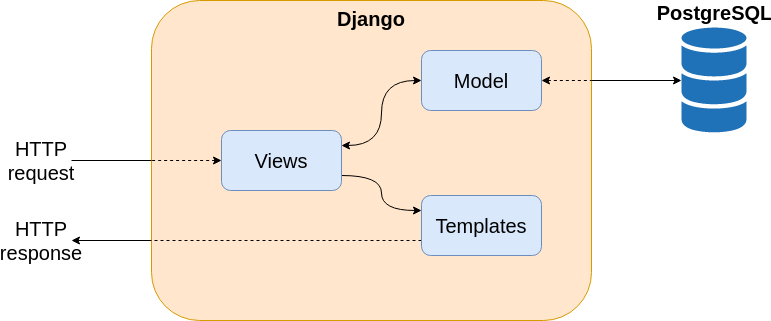
\includegraphics[width=12cm, keepaspectratio]{img/django.png}
  \caption{Arquitectura Django.}\label{fig:django}
\end{figure}

\subsubsection{Directorios y ficheros}
\label{subsubsec:django_directorios}

En la figura~\ref{fig:directorios} se pueden observar los directorios y ficheros que componen la parte Django de la aplicación. Los ficheros y directorios más importantes y sus funciones son los siguientes:

\begin{itemize}
	\item \textbf{models.py}: Define el modelo de datos a utilizar en la base de datos de la aplicación. Dentro de la arquitectura MVT de Django, pertenece a \textit{Model}.
	\item \textbf{views.py}: En él se definen las vistas encargadas de leer y procesar el contenido de las peticiones HTTP realizadas a la aplicación para después realizar las acciones correspondientes.
	Como su propio nombre indica, se encuentra dentro de la parte \textit{Views} definida en el modelo de arquitectura MVT.
	\item \textbf{urls.py}: A través de este fichero se gestiona el acceso a los recursos (URLs) de la aplicación.
	En él se indican, mediante el uso de expresiones regulares, los recursos que son accesibles en la aplicación y se asigna a cada uno una función definida en el fichero views.py. Junto a views.py, pertenece a la parte \textit{Views} definida en el modelo de arquitectura MVT.
	\item \textbf{pylint\_errors.py}: Fichero que contiene las funciones encargadas de corregir los errores analizados por Pylint.
	\item \textbf{tests.py}: Fichero que contiene los tests unitarios desarrollados para comprobar que las funciones de la aplicación se comportan correctamente.
	\item \textbf{template}: Directorio que contiene las plantillas HTML que van a formar el cuerpo de la respuesta HTTP que se da al cliente. En su interior se encuentran los directorios \textit{es}, que contiene las plantillas en castellano, \textit{en}, que contienen las plantillas en inglés e \textit{images}, que contiene las imágenes utilizadas por las plantillas HTML. Tambien se encuentra el fichero \textit{themes.css}, que actúa como hoja de estilo para toda la aplicación. Los ficheros y directorios de su interior confirman la parte \textit{Templates} del modelo de arquitectura MVT.
\end{itemize}

\begin{figure}
  \centering
  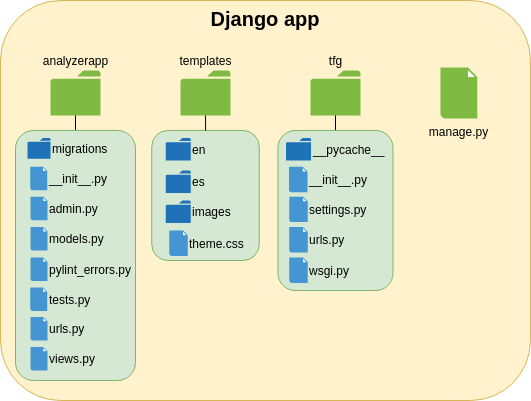
\includegraphics[height=8cm, keepaspectratio]{img/directorios.png}
  \caption{Directorios y ficheros de Django.}\label{fig:directorios}
\end{figure}

\subsubsection{Recursos}
\label{subsubsec:django_recursos}
Los recursos accesibles definidos en \textit{urls.py} son los siguientes:
\begin{itemize}
	\item \textbf{/}: Recurso que devuelve la página principal de la aplicación.
	Llama a la vista \textit{views.main}.
	\item \textbf{/repo/id}: Muestra la información correspondiente al repositorio del id indicado y permite llevar a cabo el análisis del mismo y la corrección de los errores detectados.
	Llama a la vista \textit{views.repo}.
	\item \textbf{/list}: Muestra la información de todas las Pull-Requests/Merge-Requests que se han llevado a cabo.
	Llama a la vista \textit{views.list}.
	\item \textbf{/error-list}: Muestra dos gráficas, una con el recuento del número de veces que se ha corregido cada error y otra con el estado actual de las Pull-Requests/Merge-Requests realizadas.
	Llama a la vista \textit{views.error\_list}.
	\item \textbf{/guide}: Contiene una guía de uso de la aplicación. 
	Llama a la vista \textit{views.guide}.
	\item \textbf{/contact}: Muestra los datos de contacto.
	Llama a la vista \textit{views.contact}.
	\item \textbf{/es}: Cambia el idioma del usuario a castellano.
	Llama a la vista \textit{views.es}.
	\item \textbf{/en}: Cambia el idioma del usuario a inglés.
	Llama a la vista \textit{views.en}.
\end{itemize}

\subsubsection{Vistas}
\label{subsubsec:django_vistas}
 Las vistas de Django definidas en el fichero \textit{views.py} y sus funciones son las siguientes:
\begin{itemize}
	\item \textbf{main}: Si recibe un GET, devuelve el template \textit{main.html}.
	Mientras que si recibe un POST evalúa el contenido introducido en el formulario y, dependiendo de éste, pueden producirse varias situaciones:
	\begin{itemize}
		\item El contenido está vacío: se devuelve el template \textit{error.html}.
		\item El contenido no corresponde a un repositorio: se devuelve el template \textit{error\_repo.html}.
		\item Se ha introducido un repositorio que tiene una Pull-Request/Merge-Request realizada por la aplicación en estado abierto: se devuelve el template \textit{request\_exists.html}.
		\item Se ha introducido un repositorio sin ninguna Pull-Request/Merge-Request realizada por la aplicación en estado abierto: se redirige al recurso \textit{/repo/id}.
	\end{itemize}
	\item \textbf{repo}: Si recibe un GET, devuelve el template \textit{repo\_data.html}.
	Mientras que si recibe un POST evalúa el nombre del formulario que ha realizado la petición y, dependiendo de éste, pueden producirse varias situaciones:
	\begin{itemize}
		\item \textit{pylint}: Se lanza la función asíncrona que ejecuta el análisis del código utilizando Pylint y se devuelve el template \textit{running\_pylint.html}.
		\item \textit{running}: Espera un tiempo determinado y comprueba si la función asíncrona que ejecuta el análisis del código ha finalizado. En caso de que haya finalizado, devuelve el template \textit{repo\_data\_pylint.html}, mientras que si el análisis sigue en ejecución, devuelve otra vez el template \textit{running\_pylint.html}.
		\item \textit{fix\_errors}: Se lanza la función asíncrona que ejecuta la corrección de los errores detectados por Pylint y se devuelve el template \textit{fixing\_errors.html}.
		\item \textit{fixing}: Espera un tiempo determinado y comprueba si la función asíncrona que ejecuta la corrección del código ha finalizado. En caso de que haya finalizado, devuelve el template \textit{repo\_data\_success.html}, mientras que si el análisis sigue en ejecución, devuelve otra vez el template \textit{fixing\_errors.html}.
	\end{itemize}
	\item \textbf{list}: Obtiene la lista de repositorios analizados y devuelve el template \textit{list.html}. 
	\item \textbf{error\_list}: Obtiene el número de errores corregidos y el estado de las Pull-Requests/Merge-Requests realizadas y  devuelve el template \textit{error\_list.html}.
	\item \textbf{guide}: Devuelve el template \textit{guide.html}.
	\item \textbf{contact}: Devuelve el template \textit{contact.html}.
	\item \textbf{es}: Cambia el valor de la variable de sesión correspondiente al idioma para visualizar el sitio en castellano y redirige a la página principal.
	\item \textbf{en}: Cambia el valor de la variable de sesión correspondiente al idioma para visualizar el sitio en inglés y redirige a la página principal.
\end{itemize}
Además, todas las vistas tienen una parte común al recibir un GET: comprueban el estado de las Pull-Requests/Merge-Requests para actualizarlo en la base de datos si éste ha cambiado y también comprueban el valor de la variable de sesión correspondiente al idioma para así devolver las templates en castellano o en inglés según corresponda.

\subsubsection{Templates}
\label{subsubsec:django_templates}
Las plantillas HTML del proyecto se encuentran divididas en los directorios \textit{templates/en} y \textit{templates/es}. Las plantillas de un directorio son prácticamente iguales a las del otro, diferenciándose únicamente en el idioma de los textos.

Las plantillas y sus contenidos son las siguientes:
\begin{itemize}
	\item \textbf{base.html}: Fichero base que extienden el resto de plantillas. Define el banner, el fondo y el menú lateral y su funcionamiento mediante un script.
	\item \textbf{main.html}: Contiene el formulario de introducción de repositorios.
	\item \textbf{error.html}: Muestra el mensaje de error que se le pase como parámetro.
	\item \textbf{error\_repo.html}: Muestra un mensaje de error indicando que el formulario no se ha rellenado con una URL que pertenezca a un repositorio.
	\item \textbf{request\_exists.html}: Informa de que ya existe una Pull-Request/Merge-Request abierta para el repositorio indicado y muestra una tabla con la información de dicho repositorio y la petición realizada.
	\item \textbf{repo\_data.html}: Muestra una tabla con la información del repositorio introducido y un formulario para ejecutar el análisis con Pylint. Dicho formulario es sustituido por una imagen en movimiento al ser pulsado.
	\item \textbf{running\_pylint.html}: Muestra una tabla con la información del repositorio introducido y una imagen y mensaje informando de que se está realizando el análisis. Mediante un script, al terminar la carga realiza una redirección ejecutando un POST al recurso \textit{/repo/id} con un body con el mensaje ``running''.
	\item \textbf{repo\_data\_pylint.html}: Muestra una tabla con la información del repositorio introducido, los errores detectados en el análisis realizado por Pylint y un botón para ejecutar la corrección. Mediante pestañas se puede filtrar para ver todos los errores o sólo los errores corregibles por la aplicación.
	\item \textbf{fixing\_errors.html}: Muestra una tabla con la información del repositorio introducido y una imagen y mensaje informando de que se está realizando la corrección del código. Mediante un script, al terminar la carga realiza una redirección ejecutando un POST al recurso \textit{/repo/id} con un body con el mensaje ``fixing''.
	\item \textbf{repo\_data\_success.html}:  Muestra una tabla con la información del repositorio introducido y añade una nueva fila con el enlace a la Pull-Request/Merge-Request realizada.
	\item \textbf{list.html}: Muestra una tabla con la lista de las Pull-Requests/Merge-Requests realizadas por la aplicación. Mediante pestañas se puede realizar un filtrado según el estado de cada una.
	\item \textbf{error\_list.html}: Hace uso de la librería de JavaScript Chart.js~\ref{sec:chartjs} para representar dos gráficas, una con el recuento de errores y otra con el estado de las Pull-Requests/Merge-Requests realizadas.
	\item \textbf{guide.html}: Contiene un resumen sobre la aplicación, una breve guía de uso definiendo cada una de las páginas y una tabla con los errores detectados por Pylint que son corregibles por la aplicación.
	\item \textbf{contact.html}: Contiene los datos de contacto.
	\item \textbf{theme.css}: Hoja de estilo para personalizar el aspecto de los elementos HTML de la aplicación.
\end{itemize}

\subsection{Errores de Pylint}
\label{subsec:errores}

En el fichero \textit{pylint\_errors.py} se definen qué errores detectados por Pylint van a ser corregidos y cómo va a llevarse a cabo la corrección. 
El listado de errores corregibles por la aplicación se puede visualizar en la tabla~\ref{tabla:errores}.

Pylint indica dónde aparecen los errores mediante el número de línea en el que se encuentran, por lo que para realizar la corrección se ha hecho uso de placeholders que se añaden al código e indican si una determinada línea tiene un error y de qué tipo es.
De esta forma no se cambian las líneas de posición y se evitan posibles modificaciones en las líneas incorrectas.
Una vez terminada la colocación de los placeholders para todo el código, se vuelve a escanear el fichero línea por línea y se aplica la corrección correspondiente para cada placeholder encontrado.
\begin{table}
 \begin{center}
  \begin{tabular}{ | l | c | c |}
    \hline
    \textbf{Error ID} & \textbf{Error Name} & \textbf{Message} \\ \hline
    C0303 & trailing-whitespace & \makecell[l]{Trailing whitespace. Used when there is whitespace\\between the end of a line and the newline.} \\ \hline
    C0304 & missing-final-newline & \makecell[l]{Final newline missing. Used when the last line in\\a file is missing a newline.} \\ \hline
    C0321 & multiple-statements & \makecell[l]{More than one statement on a single line. Used when\\more than on statement are found on the same line.} \\ \hline
    C0326 & bad-whitespace & \makecell[l]{\%s space \%s \%s \%s. Used when a wrong number of spaces\\is used around an operator, bracket or block opener.} \\ \hline
    C0410 & multiple-imports & \makecell[l]{Multiple imports on one line (\%s). Used when import\\statement importing multiple modules is detected.} \\ \hline
    C0411 & wrong-import-order & \makecell[l]{\%s should be placed before \%s. Used when PEP8\\import order is not respected (standard imports first, then\\third-party libraries, then local imports)} \\ \hline
    C0413 & wrong-import-position & \makecell[l]{Import "\%s" should be placed at the top of the\\module. Used when code and imports are mixed} \\ \hline
    W0404 & reimported & \makecell[l]{Reimport \%r (imported line \%s). Used when a module\\is reimported multiple times.} \\ \hline
    W0611 & unused-import & \makecell[l]{Unused \%s. Used when an imported module or\\variable is not used.} \\ \hline
  \end{tabular}
  \label{tabla:errores}
  \caption{Errores detectados por Pylint corregibles por la aplicación.}
 \end{center}
\end{table}

\subsection{Base de datos}
\label{subsec:diseño_bbdd}

La estructura de la base de datos queda definida en el fichero \textit{models.py} de Django y tiene la forma representada en la figura~\ref{fig:models}.
Está compuesta por las siguientes tablas:
\begin{itemize}
	\item \textbf{Errors}: Contiene la información relativa a todos los errores detectables por Pylint y si son corregibles o no por la aplicación.
	\item \textbf{Repository}: Almacena la información de todos los repositorios que han sido analizados por la aplicación y las Pull-Requests/Merge-Requests que se han llevado a cabo.
	\item \textbf{All\_errors\_repo}: Guarda los errores que se han detectado en cada repositorio.
	\item \textbf{Fixed\_errors\_repo}: Guarda los errores que se han detectado en cada repositorio y además han sido corregidos por la aplicación.
	\item \textbf{All\_errors\_count}:  Almacena el número de veces que se ha detectado cada error.
	\item \textbf{Fixed\_errors\_count}: Almacena el número de veces que se ha corregido cada error.
\end{itemize}

Es una base de datos PostgreSQL provisionada por Heroku y externa a la aplicación Django.

\begin{figure}
  \centering
  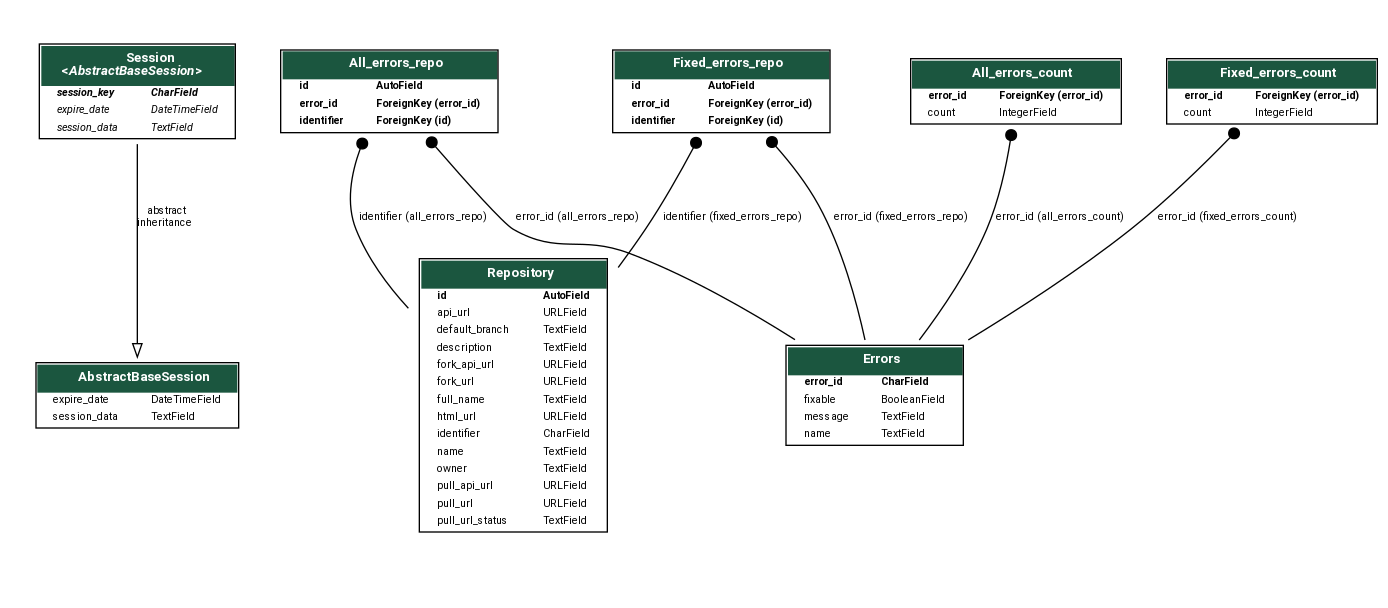
\includegraphics[width=16cm, keepaspectratio]{img/models.png}
  \caption{Modelo de datos.}\label{fig:models}
\end{figure}

\subsection{Despliegue}
\label{subsec:diseño_despliegue}

El despliegue de la aplicación se ha configurado para que se lleve a cabo de manera automática mediante el uso de las GitHub Actions y Heroku.

\subsubsection{Github}
\label{subsubsec:despliegue_github}

Cuando se realiza un push y se suben los nuevos commits a GitHub, se ejecutan automáticamente las GitHub Actions definidas en el directorio \textit{/.github/workflows/}.

El fichero \textit{main.yml}, ubicado en dicho directorio, hace uso de la GitHub Action \textit{akhileshns/heroku-deploy@v3.12.12}~\cite{herokudeploy}, logrando así que la aplicación se despliegue automáticamente en Heroku cada vez que se hace push al repositorio que contiene el código.

\subsubsection{Heroku}
\label{subsubsec:despliegue_heroku}
Para llevar a cabo el despliegue de la aplicación en Heroku es necesaria la configuración de dos ficheros, \textit{Procfile} y \textit{requirements.txt}.

\textit{Procfile} especifica los comandos que se van a ejecutar durante el despliegue de la aplicación en Heroku.
Para esta aplicación se especifica que se deben realizar las migraciones del modelo de datos en el momento del lanzamiento, o \textit{release}, por si se hubiese llevado a cabo alguna modificación en \textit{models.py}, y se ejecuta el comando \textit{runserver} como un proceso de tipo web para que sea accesible y pueda recibir peticiones HTTP desde fuera de Heroku.

El fichero \textit{requirements.txt} hace que Heroku identifique automáticamente la aplicación como una aplicación desarrollada en Python y en su interior se definen las dependencias, incluyendo la versión, que deben ser instaladas antes del arranque de la aplicación en Heroku.
Para esta aplicación \textit{requirements.txt} contiene paquetes Python como \textit{Django}, \textit{Pylint}, o \textit{requests}, entre otros.


%%%%%%%%%%%%%%%%%%%%%%%%%%%%%%%%%%%%%%%%%%%%%%%%%%%%%%%%%%%%%%%%%%%%%%%%%%%%%%%%
%%%%%%%%%%%%%%%%%%%%%%%%%%%%%%%%%%%%%%%%%%%%%%%%%%%%%%%%%%%%%%%%%%%%%%%%%%%%%%%%
% EXPERIMENTOS Y VALIDACIÓN %
%%%%%%%%%%%%%%%%%%%%%%%%%%%%%%%%%%%%%%%%%%%%%%%%%%%%%%%%%%%%%%%%%%%%%%%%%%%%%%%%

\cleardoublepage
\chapter{Experimentos y validación}

\section{Tests unitarios}
\label{sec:tests}
Para comenzar las pruebas del correcto funcionamiento de la aplicación se ha hecho uso de la herramienta de tests unitarios incluida en Django.
Dichos tests unitarios se encuentran en el fichero \textit{/analyzerapp/tests.py} y están diseñados para comprobar que las funciones correspondientes a cada error son capaces de situar correctamente el placeholder indicado en las líneas afectadas y que las funciones que corrigen los errores al encontrar un placeholder son capaces de hacerlo correctamente.
\begin{figure}[h]
  \centering
  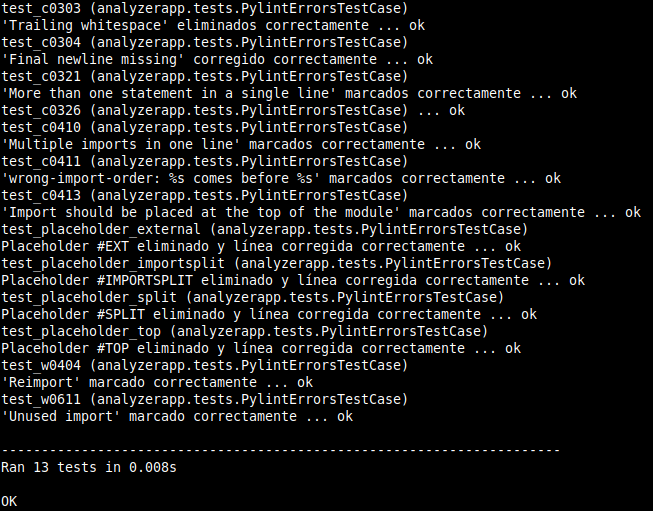
\includegraphics[width=10cm, keepaspectratio]{img/tests.png}
  \caption{Salida de la ejecución de los tests unitarios en Django.}\label{fig:tests}
\end{figure}

La salida de la ejecución de los tests unitarios desde el propio Django puede ser observada en la figura~\ref{fig:tests}. En ella se refleja que la ejecución de los tests unitarios es exitosa tanto para los 9 tests correspondientes a las funciones que añaden los placehoolders, como para los 4 tests correspondientes a la corrección de los errores y borrado de los placeholders.


%%%%%%%%%%%%%%%%%%%%%%%%%%%%%%%%%%%%%%%%%%%%%%%%%%%%%%%%%%%%%%%%%%%%%%%%%%%%%%%%
%%%%%%%%%%%%%%%%%%%%%%%%%%%%%%%%%%%%%%%%%%%%%%%%%%%%%%%%%%%%%%%%%%%%%%%%%%%%%%%%
% RESULTADOS %
%%%%%%%%%%%%%%%%%%%%%%%%%%%%%%%%%%%%%%%%%%%%%%%%%%%%%%%%%%%%%%%%%%%%%%%%%%%%%%%%

\cleardoublepage
\chapter{Resultados}
%TODO
En este capítulo se incluyen los resultados de tu trabajo fin de grado.

Si es una herramienta de análisis lo que has realizado, aquí puedes poner ejemplos de haberla utilizado para que se vea su utilidad.


%%%%%%%%%%%%%%%%%%%%%%%%%%%%%%%%%%%%%%%%%%%%%%%%%%%%%%%%%%%%%%%%%%%%%%%%%%%%%%%%
%%%%%%%%%%%%%%%%%%%%%%%%%%%%%%%%%%%%%%%%%%%%%%%%%%%%%%%%%%%%%%%%%%%%%%%%%%%%%%%%
% CONCLUSIONES %
%%%%%%%%%%%%%%%%%%%%%%%%%%%%%%%%%%%%%%%%%%%%%%%%%%%%%%%%%%%%%%%%%%%%%%%%%%%%%%%%

\cleardoublepage
\chapter{Conclusiones}
\label{chap:conclusiones}
%TODO

\section{Consecución de objetivos}
\label{sec:consecucion-objetivos}

Esta sección es la sección espejo de las dos primeras del capítulo de objetivos, donde se planteaba el objetivo general y se elaboraban los específicos.

Es aquí donde hay que debatir qué se ha conseguido y qué no. 
Cuando algo no se ha conseguido, se ha de justificar, en términos de qué problemas se han encontrado y qué medidas se han tomado para mitigar esos problemas.

Y si has llegado hasta aquí, siempre es bueno pasarle el corrector ortográfico, que las erratas quedan fatal en la memoria final.
Para eso, en Linux tenemos aspell, que se ejecuta de la siguiente manera desde la línea de \emph{shell}:

\begin{verbatim}
  aspell --lang=es_ES -c memoria.tex
\end{verbatim}

\section{Aplicación de lo aprendido}
\label{sec:aplicacion}

Aquí viene lo que has aprendido durante el Grado/Máster y que has aplicado en el TFG/TFM. Una buena idea es poner las asignaturas más relacionadas y comentar en un párrafo los conocimientos y habilidades puestos en práctica.

\begin{enumerate}
  \item a
  \item b
\end{enumerate}


\section{Lecciones aprendidas}
\label{sec:lecciones_aprendidas}

Aquí viene lo que has aprendido en el Trabajo Fin de Grado/Máster.

\begin{enumerate}
  \item Aquí viene uno.
  \item Aquí viene otro.
\end{enumerate}


\section{Trabajos futuros}
\label{sec:trabajos_futuros}

Ningún proyecto ni software se termina, así que aquí vienen ideas y funcionalidades que estaría bien tener implementadas en el futuro.

Es un apartado que sirve para dar ideas de cara a futuros TFGs/TFMs.


%%%%%%%%%%%%%%%%%%%%%%%%%%%%%%%%%%%%%%%%%%%%%%%%%%%%%%%%%%%%%%%%%%%%%%%%%%%%%%%%
%%%%%%%%%%%%%%%%%%%%%%%%%%%%%%%%%%%%%%%%%%%%%%%%%%%%%%%%%%%%%%%%%%%%%%%%%%%%%%%%
% APÉNDICE(S) %
%%%%%%%%%%%%%%%%%%%%%%%%%%%%%%%%%%%%%%%%%%%%%%%%%%%%%%%%%%%%%%%%%%%%%%%%%%%%%%%%

\cleardoublepage
\appendix
\chapter{Manual de usuario}
\label{app:manual}
%TODO
Esto es un apéndice.
Si has creado una aplicación, siempre viene bien tener un manual de usuario.
Pues ponlo aquí.

%%%%%%%%%%%%%%%%%%%%%%%%%%%%%%%%%%%%%%%%%%%%%%%%%%%%%%%%%%%%%%%%%%%%%%%%%%%%%%%%
%%%%%%%%%%%%%%%%%%%%%%%%%%%%%%%%%%%%%%%%%%%%%%%%%%%%%%%%%%%%%%%%%%%%%%%%%%%%%%%%
% BIBLIOGRAFIA %
%%%%%%%%%%%%%%%%%%%%%%%%%%%%%%%%%%%%%%%%%%%%%%%%%%%%%%%%%%%%%%%%%%%%%%%%%%%%%%%%

\cleardoublepage

% Las siguientes dos instrucciones es todo lo que necesitas
% para incluir las citas en la memoria
\bibliographystyle{abbrv}
\bibliography{memoria}  % memoria.bib es el nombre del fichero que contiene
% las referencias bibliográficas. Abre ese fichero y mira el formato que tiene,
% que se conoce como BibTeX. Hay muchos sitios que exportan referencias en
% formato BibTeX. Prueba a buscar en http://scholar.google.com por referencias
% y verás que lo puedes hacer de manera sencilla.
% Más información: 
% http://texblog.org/2014/04/22/using-google-scholar-to-download-bibtex-citations/

\end{document}
